%%%%%%%%%%%%%%%%%%%%%%%%%%%%%%%%%%%%%%%%%%%%%%%%%%%%%%%%%%%%%%%%%%%
%                                                                 %
%                            CHAPTER                              %
%                                                                 %
%%%%%%%%%%%%%%%%%%%%%%%%%%%%%%%%%%%%%%%%%%%%%%%%%%%%%%%%%%%%%%%%%%%

\chapter{Introduction}
Deep learning-based object detection on images is a hot topic for researchers and interest in machine learning is steadily growing among miscellaneous businesses. Facial recognition is one of the many applications machine learning has to offer. A face recognition algorithm tries to recognize faces of the same person. Faces are very unique parts of our body, thus face matching can be used as a means to do biometric authentication. In this case, a client sends a picture containing their face to an external service which grants the client access if the face is similar to the one stored in the database.

More and more users are concerned about their privacy and the security of their data stored and processed on servers. Not only are they afraid of malicious hackers stealing their sensitive data, they also fear the servers operator will use their data for purposes other than the user agreed to. Big corporations have been found guilty of collecting user data for unethical purposes (source: \cite{cadwalladr2018revealed}).

Secure multiparty computation (MPC) is a subfield of cryptography, making it possible for a party to run an algorithm on confidential data, that is supposed to stay unknown even to the party running the algorithm. There exist different methods to perform privacy-preserving computations, MPC is the one we will use.

Secure Multiparty Computation and Machine Learning aren't new concepts, in fact they exist for over 40 years. But with the rise of big data and processing power lately, there has been an increase in research into these fields.

Because of these concerns researchers are looking for technologies to enhance the privacy of the user during the processing of it's data on a server.

Onespan\footnote{Onespan's official website: \url{https://www.onespan.com}} (formerly VASCO Data Security International, Inc.) is a global company were most of our research was done. Onespan offers a series of security and authentication products and technologies and specializes in digital identity and anti-fraud solutions. The company continues to be active in research and innovation in different fields of technology, especially cryptography and data science.

In this thesis we study the applicability of MPC protocols on deep learning-based face matching algorithms and try to implement a privacy-preserving face matching algorithm.

\section{Problem}
The use of third party MLaaS (Machine Learning as a Service) providers or any cloud computing solution, as processing power for an image classification task, raises privacy concerns as sensitive images of users need to be sent to servers running an instance of the neural network.

It's important to note that the transport of the image from the client to the server is deemed to be secure, since the parties can make use of reliable HTTPS (Hypertext Transfer Protocol Secure) connections.

The user's images, however, are stored in plaintext \footnote{plaintext or cleartext are common cryptographic terms for unencrypted data.} on the server, as well as the computed output of the image.

Furthermore the whole design of the neural network including all trained parameters needs to be stored on the servers of the third party, for the image classifier to function. Both of these remote processing solutions require a considerably amount of trust in the third party. Since the third party could potentially exploit the user data for commercial purposes or even steal the intellectual property of the image classifier. Of course most cloud computing service providers are not inherently malicious. But as long as the user's data is stored in cleartext on the server, there is a risk that the service provider could turn malicious. Or even worse, hackers could break in to the server and breach the confidential user data.

In this thesis we try to tackle the need to trust a third party MLaaS provider. We want it to compute an encrypted image on an obfuscated neural network to output a correct encrypted result. This encrypted result shall be sent to the client, which will then decrypt it.\\

In figure \ref{fig:workflow} a high-level workflow of secure face recognition is shown. The MPC protocol works for three parties, who each have their own computing instance connected to the MPC network and the client. The workflow commences by acquiring an image of the clients face, this can be done by taking a photograph with the front-facing camera of the clients smartphone. The client then performs secret sharing on the image and sends the shared secret to the participating parties. The parties receive their shares and jointly compute the output of the face recognition model on the given shared image of the face. The face recognition model can be public or secret. In the case of a secret model, the secret shares of the weights and biases need to be sent to the participating parties as well. Note that this only has to be done once, during initialization. After the computation is finished, the parties send their resulting secret shares to the client. The client interpolates the shares to find the secret values determining if her face matches or not.

\begin{figure}[H]
  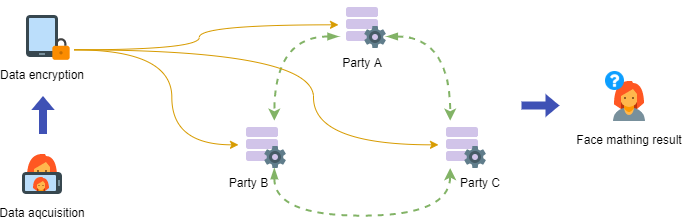
\includegraphics[width=\linewidth]{fig/workflow.png}
  \caption{Workflow of secure face matching}
  \label{fig:workflow}
\end{figure}

This protocol ensures that the client is the only one having knowledge about the cleartext of the image and the output of the face recognition algorithm. This protocol also offers an obfuscation of the model's parameters, the parties and the client have no knowledge about the parameters if the owner of the model uses secret sharing to send the parameters to the parties.\\

Before we begin specifying our hypotheses, lets define some frequently occurring terms:

\begin{itemize}
  \item Encryption: the process of converting data into a code, to ensure confidentiality and prevent unauthorized access.
  \item Privacy-preserving/secure algorithms: Algorithms that allow computation of private data, while preserving privacy.
  \item Face matching algorithm: Set of rules that a computer uses to compare two faces, to determine whether there is a match.
\end{itemize}

\section{Hypothesis}
\label{chapter:hypothesis}
\paragraph{How can we securely compute the inference of a deep learning-based facial recognition neural network?}\mbox{} \\
With the use of MPC protocols we can implement methods such that we can compute a whole face recognition convolutional neural network on an encrypted image of a face. This preserves the privacy of the user while allowing the computation to be outsourced to an untrusted third party.
\paragraph{How can we optimize the secure facial recognition task to run more efficiently?}\mbox{}
\\
We predict a drastic decrease in performance when running inference on the privacy-preserving neural network, because MPC is a protocol over a network of parties the computational time will not be the only factor to account for. We will try to find performance optimizations along the way of implementing a proof of concept by looking at existing optimization concepts for MPC as well as optimization solutions for neural networks.
